% ==============================================================================
% Section 1.12: Chapter Summary
% ==============================================================================

\section{Chapter Summary}
\label{sec:chapter_summary}

\subsection{What This Chapter Has Established}

This chapter presented a unified structural interpretation of weak-sector
phenomenology within the thick-brane framework of Elastic Diffusive Cosmology.
The core achievements are:

\subsubsection{A Unified Pipeline}

All weak decays pass through the same three-stage pipeline defined in
Section~\ref{sec:unified_pipeline}: Absorption $\to$ Dissipation $\to$ Release.
The differences between particles arise from their ontological category
(\S\ref{sec:ontology}) and kinematic thresholds, not from fundamentally
different mechanisms.

\subsubsection{Mechanistic Interpretation of Channel Selection}

The projection operator $\mathcal{P}_{\text{frozen}}$ (Section~\ref{sec:unified_pipeline})
transforms ``why does this decay happen?'' into ``what projection gates are open?''---providing
a mechanistic language for decay selection rules.

\subsubsection{Ontological Classification}

Particles occupy distinct positions in the 5D geometry:
\begin{itemize}[nosep]
  \item \textbf{Bulk-core junctions}: Neutron, proton (hadronic sector)
  \item \textbf{Brane-dominant modes}: Electron, muon, tau (leptonic sector)
  \item \textbf{Edge modes}: Neutrinos (at bulk-brane interface)
  \item \textbf{Composites}: Pions (junction-pair configurations)
\end{itemize}

This classification is not merely taxonomic; it determines dynamical behavior.

\subsubsection{Explicit Falsifiability}

Each case study includes explicit falsifiability hooks. The framework is
empirically vulnerable: if observations contradict the structural predictions,
the framework fails.

\subsection{Open Problems}

The complete list of open problems is consolidated in Section~\ref{sec:epistemic_map}.
The top priorities for this chapter are:
\begin{itemize}[nosep]
  \item Derive $\tau_n$ from junction dynamics (Chapter~2 provides 6\% accuracy)
  \item Derive $G_F$ from mediator integration (Chapter~3)
  \item Derive lepton mass hierarchy from brane mode spectrum
  \item Derive neutrino properties from edge-mode dynamics
\end{itemize}

\subsection{Comparison with Standard Model}

\begin{center}
\begin{tabular}{p{4cm}p{5cm}p{5cm}}
\toprule
\textbf{Aspect} & \textbf{Standard Model} & \textbf{EDC Interpretation} \\
\midrule
Weak interactions & Fundamental $SU(2)_L \times U(1)_Y$ gauge theory &
Effective description of thick-brane dynamics \\
\addlinespace
$G_F$ origin & $W$-boson exchange with $g^2/M_W^2$ &
Mediator integration with overlap suppression \\
\addlinespace
Chirality & V$-$A structure by construction &
Boundary condition effect at observer edge \\
\addlinespace
Neutrino mass & Requires extension (seesaw, etc.) &
Natural from edge-mode spectrum \\
\addlinespace
Hierarchy problem & Fine-tuning puzzle &
Geometric origin (overlap suppression) \\
\bottomrule
\end{tabular}
\end{center}

EDC does not contradict the Standard Model; it provides a structural context
in which SM parameters have geometric meaning.

\subsection{The Research Program}

The work outlined in this chapter defines a research program with clear
milestones:

\paragraph{Near-term (analytical).}
\begin{itemize}[nosep]
  \item Solve the thick-brane mode equation for the lowest modes
  \item Compute overlap integrals for the mediator exchange
  \item Derive boundary conditions for spinor modes
\end{itemize}

\paragraph{Medium-term (quantitative).}
\begin{itemize}[nosep]
  \item Obtain numerical values for lifetimes and compare to experiment
  \item Compute $G_F$ and compare to measured value
  \item Derive helicity suppression factor from boundary conditions
\end{itemize}

\paragraph{Long-term (extensions).}
\begin{itemize}[nosep]
  \item Extend to quark sector and hadronic weak decays
  \item Connect to CP violation and matter-antimatter asymmetry
  \item Investigate cosmological implications (baryogenesis, leptogenesis)
\end{itemize}

% ==============================================================================
% Forward to Chapter 2: The Z₆ Program
% ==============================================================================

\subsection{\texorpdfstring{Forward to Chapter 2: The $\mathbb{Z}_6$ Program}{Forward to Chapter 2: The Z6 Program}}

Several questions raised in this chapter receive definitive answers in
\textbf{Chapter~2: The $\mathbb{Z}_6$ Program}. Specifically:

\begin{itemize}[nosep]
  \item \textbf{Why is the proton stable?} Chapter~2 proves that the proton Y-junction
        is a $\mathbb{Z}_3$ fixed point of the hexagonal brane symmetry---a topological
        energy minimum with positive Hessian.
  \item \textbf{Why 120° Steiner angles?} The Steiner geometry is not assumed but
        \emph{derived} from $\mathbb{Z}_6$-invariant boundary conditions.
  \item \textbf{Why is the neutron unstable?} Chapter~2 identifies the neutron as a
        lattice \emph{dislocation}---a metastable defect that relaxes via $\beta$-decay.
  \item \textbf{Why color confinement?} The $\mathbb{Z}_3$ subgroup of $\mathbb{Z}_6$
        provides topological confinement; explicit $SU(3)$ link variables are constructed.
\end{itemize}

\noindent
The [P] postulates of this chapter become [Dc] derived consequences in Chapter~2.

\medskip

\begin{center}
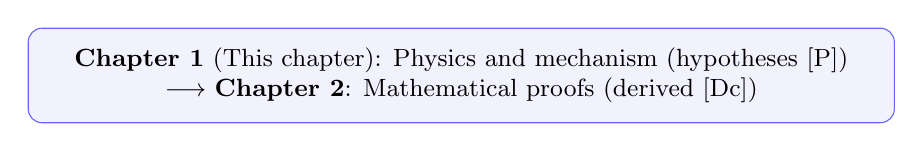
\begin{tikzpicture}
\node[rectangle, rounded corners=5pt, draw=blue!60, fill=blue!5,
      minimum width=11cm, minimum height=1.2cm, font=\small, align=center]
{
\textbf{Chapter 1} (This chapter): Physics and mechanism (hypotheses [P])\\
$\longrightarrow$ \textbf{Chapter 2}: Mathematical proofs (derived [Dc])
};
\end{tikzpicture}
\end{center}

% NOTE: Consolidated Open Questions are in Section 1.11 (sec:epistemic_map)
% This summary only provides a brief forward reference.

% ==============================================================================
% Closing Remarks
% ==============================================================================

\subsection{Closing Remarks}

This chapter has presented weak-sector phenomenology not as an isolated set of
decay processes, but as manifestations of a unified geometric structure. The
thick brane provides the arena; the projection operator provides the mechanism;
the particle ontology provides the actors.

The framework is incomplete. Many quantities remain to be computed. But the
framework is \emph{well-posed}: the calculations are defined, the success
criteria are explicit, and the falsifiability conditions are stated.

This is the status of the weak-interface sector in Elastic Diffusive Cosmology:
a coherent structural interpretation awaiting quantitative completion.

\begin{center}
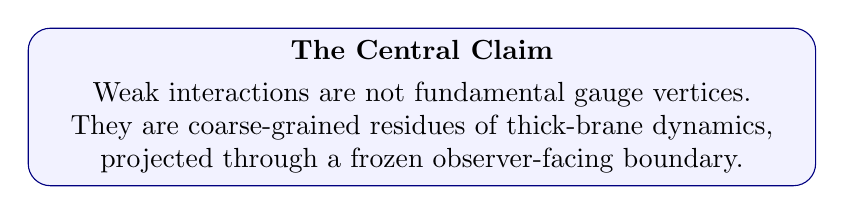
\begin{tikzpicture}
\node[rectangle, rounded corners=8pt, draw=blue!50!black, fill=blue!5,
      minimum width=10cm, minimum height=2cm, font=\normalsize, align=center]
{
\textbf{The Central Claim}\\[0.3em]
Weak interactions are not fundamental gauge vertices.\\
They are coarse-grained residues of thick-brane dynamics,\\
projected through a frozen observer-facing boundary.
};
\end{tikzpicture}
\end{center}

